\documentclass[class=report,crop=false, 12pt]{standalone}
\usepackage[screen,nosolutions]{../myscratch}
%\usepackage[screen]{../myscratch}


\begin{document}

\titre[S]{Entrée/Sortie}
%===============================

\insertvideo{delXHz33zC8}{Entrée/Sortie -- Activité 1}

\insertvideo{p9Ms6wE9X5o}{Entrée/Sortie -- Activité 2}

\insertvideo{TDo_UAN-vZ0}{Entrée/Sortie -- Activité 3}

\bigskip
\bigskip


\begin{activite}
Programme Scratch afin qu'il réagisse en fonction des commandes suivantes :
\begin{itemize}
  \item les touches de flèches font monter, descendre Scratch ou le font aller vers la gauche ou la droite,
  \item la touche \mot{m} fait jouer un son,
  \item la touche \mot{c} passe au costume suivant,
  \item la touche \mot{espace} change la couleur du stylo de $10$,
  \item la touche \mot{f} efface tout l'écran.
\end{itemize}

\medskip

\textbf{Bonus 1.} La touche \mot{r} relève le stylo, la touche \mot{s} place le stylo en position d'écriture.

\textbf{Bonus 2.} Trouve d'autres actions à contrôler avec des touches et trace de beaux dessins !

\begin{center}
  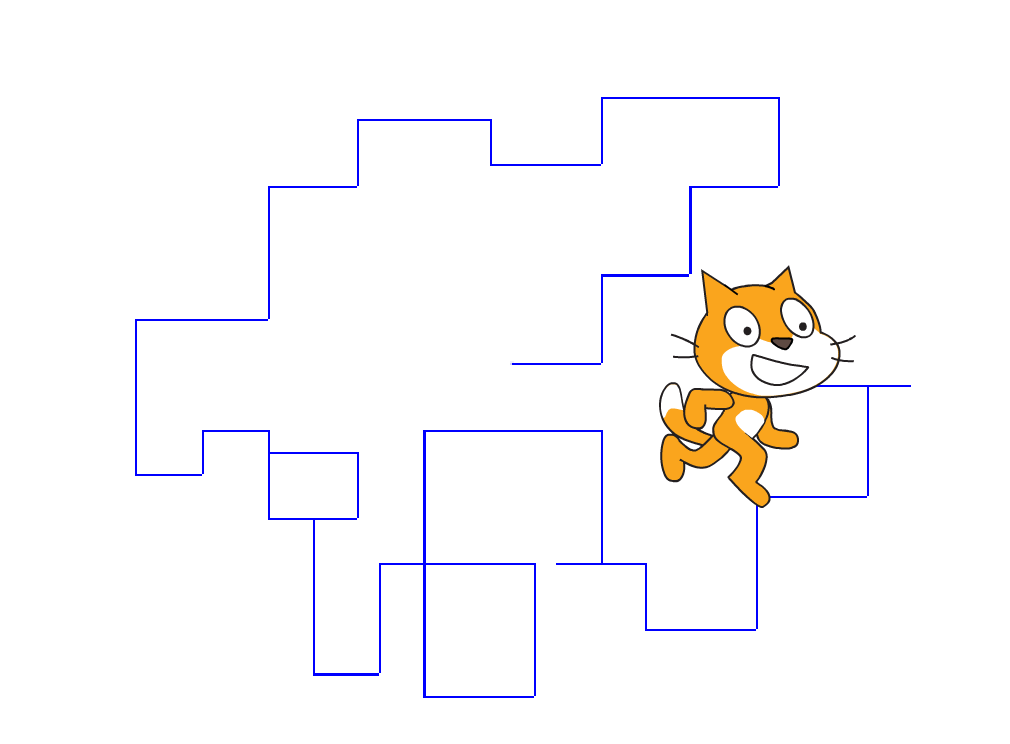
\includegraphics[width=0.7\textwidth]{ecran-05-ex1} 
\end{center}

\medskip

\textbf{Blocs utiles.}
\begin{center}
\begin{scratch}
  \blockif{si \boolsensing{touche \ovalsensing*{flèche droite} pressée ?} alors }
  { 
    \blockspace
  }
\end{scratch}
\end{center}

\end{activite}



\begin{activite}

Maintenant Scratch doit tracer un triangle en suivant les indications de l'utilisateur.

\begin{center}
  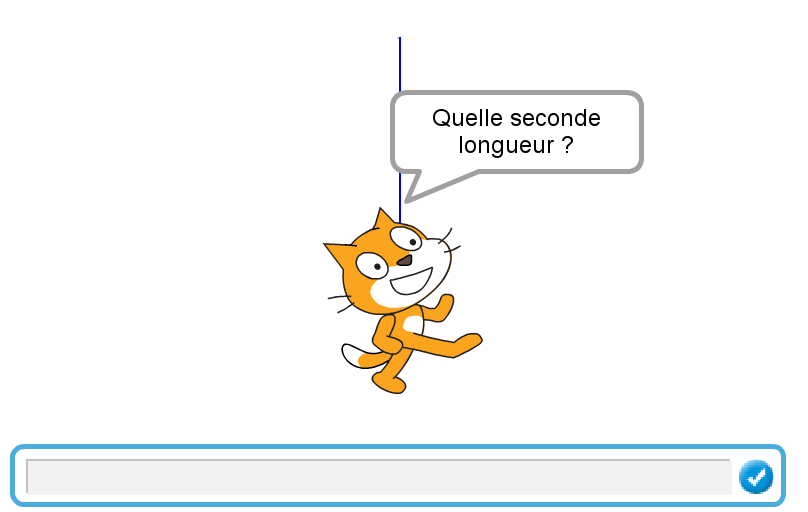
\includegraphics[width=0.6\textwidth]{ecran-05-ex2} 
\end{center}


\myfigure{0.9}{
\footnotesize  \tikzinput{figure-05-ex2}
} 


\begin{itemize}
  \item \'Etape 0. Scratch part du point $(0,100)$ et est orienté vers le Sud ($180$\textdegree).
  
  \item \'Etape 1. Demander à l'utilisateur la longueur du premier côté, puis faire avancer Scratch vers le bas du nombre de pas de la réponse.
  
  \item \'Etape 2. Demander à l'utilisateur un angle, puis orienter Scratch selon la valeur répondue.
   
  \item \'Etape 3. Demander à l'utilisateur la longueur du deuxième côté et faire avancer Scratch.
  
  \item \'Etape 4. Scratch retourne au point de départ $(0,100)$.
\end{itemize}

\bigskip

\textbf{Blocs utiles.}
Il est possible de poser une question, d'attendre la réponse, et d'utiliser la valeur répondue à l'aide de la variable \og réponse \fg{}.

\begin{center}
\begin{scratch}
  \blocksensing{demander \ovalnum{Quelle longueur ?} et attendre}
\end{scratch}
  \qquad\qquad\qquad
\ovalsensing{réponse}
\end{center}

\end{activite}



\begin{activite}
\sauteligne

\begin{enumerate}
  \item Dans un premier temps, Scratch demande le prénom de l'utilisateur et répond \og Bonjour ...\fg{} avec le prénom donné.
  
  \item Dans un second temps, Scratch demande l'âge de l'utilisateur et trace un polygone avec autant de côtés que cet âge.
  
  Par exemple si l'âge est $11$, alors Scratch exécute $11$ fois : avancer de $50$, puis tourner de $360/11$.

\end{enumerate}
\begin{center}
  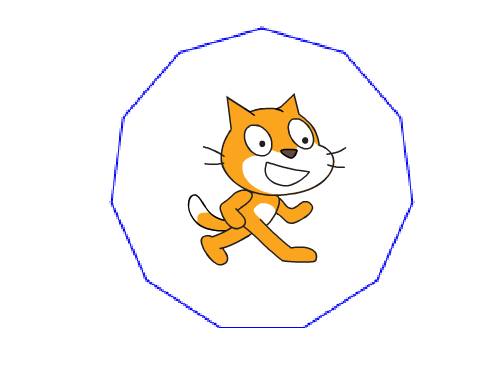
\includegraphics[width=0.5\textwidth]{ecran-05-ex3} 
\end{center}


\end{activite}


\ifx \displaysolutions \myzero
\else
\begin{code}
\setscratch{scale=\scalesolution}
\begin{minipage}[t]{0.45\textwidth}
\onesolution{Entrée/Sortie}{Activité 1}{
\begin{scratch}
  \blockinit{quand \greenflag est cliqué}
  \blockmove{aller à x: \ovalnum{0} y: \ovalnum{0}}
  \blockmove{s'orienter à \ovalnum{90}}
  \blockpen{effacer tout}
  \blockpen{stylo en position d'écriture}
  \blockinfloop{répéter indéfiniment}
  {
    \blockif{si \boolsensing{touche \ovalsensing*{flèche droite} pressée ?} alors }
    { 
      \blockmove{ajouter \ovalnum{10} à x}
    }
    \blockif{si \boolsensing{touche \ovalsensing*{flèche gauche} pressée ?} alors }
    { 
      \blockmove{ajouter \ovalnum{-10} à x}
    }
    \blockif{si \boolsensing{touche \ovalsensing*{flèche haut} pressée ?} alors }
    { 
      \blockmove{ajouter \ovalnum{10} à y}
    }
    \blockif{si \boolsensing{touche \ovalsensing*{flèche bas} pressée ?} alors }
    { 
      \blockmove{ajouter \ovalnum{-10} à y}
    }
    \blockif{si \boolsensing{touche \ovalsensing*{m} pressée ?} alors }
    { 
      \blocksound{jouer le son \ovalsound*{miaou}}
    }
    \blockif{si \boolsensing{touche \ovalsensing*{c} pressée ?} alors }
    { 
      \blocklook{costume suivant}
      \blockcontrol{attendre \ovalnum{0.1} secondes} 
    }
    \blockif{si \boolsensing{touche \ovalsensing*{espace} pressée ?} alors }
    { 
      \blockpen{ajouter \ovalnum{10} à la \ovalpen*{couleur} du stylo}
    }
    \blockif{si \boolsensing{touche \ovalsensing*{f} pressée ?} alors }
    { 
        \blockpen{effacer tout}
    }
  }
\end{scratch}
}
\end{minipage}
\begin{minipage}[t]{0.5\textwidth}
\onesolution{Entrée/Sortie}{Activité 2}{
\begin{scratch}
  \blockinit{quand \greenflag est cliqué}
  \blockmove{aller à x: \ovalnum{0} y: \ovalnum{100}}
  \blockmove{s'orienter à \ovalnum{180}}
  \blockpen{effacer tout}
  \blockpen{stylo en position d'écriture}
  \blocklook{montrer}

  \blocksensing{demander \ovalnum{Quelle première longueur ?} et attendre}
  \blockmove{avancer de \ovalsensing{réponse} pas}

  \blocksensing{demander \ovalnum{Quel angle ?} et attendre}
  \blockmove{s'orienter à \ovalsensing{réponse}}

  \blocksensing{demander \ovalnum{Quelle seconde longueur ?} et attendre}
  \blockmove{avancer de \ovalsensing{réponse} pas}

  \blockmove{aller à x: \ovalnum{0} y: \ovalnum{100}}
  \blocklook{cacher}
\end{scratch}
}

\bigskip

\onesolution{Entrée/Sortie}{Activité 3}{
\begin{scratch}
  \blockinit{quand \greenflag est cliqué}
  \blockmove{aller à x: \ovalnum{0} y: \ovalnum{-100}}
  \blockmove{s'orienter à \ovalnum{90}}
  \blockpen{effacer tout}
  \blockpen{stylo en position d'écriture}

  \blocksensing{demander \ovalnum{Quel est ton prénom ?} et attendre}
  \blocklook{dire  
     \ovaloperator{regrouper \ovalnum{ Bonjour} et \ovalsensing{réponse}}
     pendant \ovalnum{2} secondes}

  \blocksensing{demander \ovalnum{Quel âge as-tu ?} et attendre}
  \blockrepeat{répéter \ovalsensing{réponse} fois}{
    \blockmove{avancer de \ovalnum{50} pas}
    \blockmove{tourner \turnleft{} de \ovaloperator{\ovalnum{360} / \ovalsensing{réponse}} degrés}
  }
\end{scratch}
}
\end{minipage}
\end{code}
\fi


\end{document}

